\section{Data}
\subsection{Overview}
The study used 16 right-handed, healthy, English-speaking participants 
recruited through ads posted on UCLA. Out of 16 subjects, 9 were female and 
the mean age was 22 $ \pm $ 2.9 years. \cite{Tom2007LossAversion}

\subsection{Behavorial Data}
The behavioral data consists of each subject undergoing 3 trial runs for the 
``gamble'' task, in which each subject is presented with a combination of 
potential monetary gains and losses given a 50/50 chance of to win/loss. Each 
trial run consists of 86 different combinations of rewards/penalities spread 
out accross 474 seconds. Intervals between each onset of task range from 4 to 
8 seconds. Subjects were given the 4 choices in reponse to each gambling 
proposal:
\begin{enumerate}
  \item Strong Accept
  \item Weak Accept
  \item Weak Reject
  \item Strong Reject
\end{enumerate}
The choices are recorded by denoting reponse numbers 1, 2, 3, and 4, 
respectively. Furthermore, the response time for each gambling decision was 
recorded in seconds. 
\subsection{BOLD Data}
Blood-oxygen-level dependent (BOLD) imaging data were collected from each 
subject as he/she performed the gamble tasks. 240 time scans were done on each 
run with a time between each scan of 2 seconds. So total scanning time is 480 
seconds. Each scan consists of a snapshot consisting of a64 by 64 by 34 image 
matrix. 

There are also 4 model conditions, with events corresponding to 
\begin{enumerate}
  \item Task
  \item Parametric Gain
  \item Parametric Loss
  \item Distance from Indifference
\end{enumerate}

\subsection{Processing}
Before we run our analyses and fit betas to our data, we first take a few 
steps to clean the BOLD datasets. We graph the dvars (RMS of the signal 
derivatives) and the framewise displacement, and we use that in conjunction 
with the mean signal of the BOLD data to determine outliers to remove. The 
BOLD data is smoothed spatially in order to make clearer the signal in 
relation to the noise present. We also take the mean signal of the BOLD data 
across the run and plot the histogram for each run and subject to help 
manually determine a good threshold for a mask we use to isolate more active 
voxels in the brain. This helps us find beta coefficients for more relevant 
voxels. We also model and remove the linear and quadratic drift that may be 
present in the runs. 
We use subject 2 run 2 to show an example of our outlier results.

\begin{figure}[H]
    \centering
        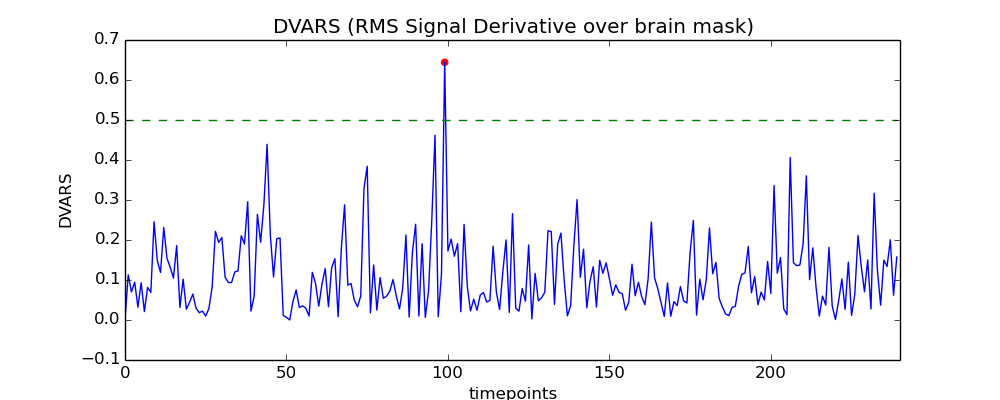
\includegraphics[scale=0.5]{figures/dvars_sub2run2.png}
    \caption{DVARS for subject 2 run 2}
\end{figure}

\begin{figure}[H]
    \centering
        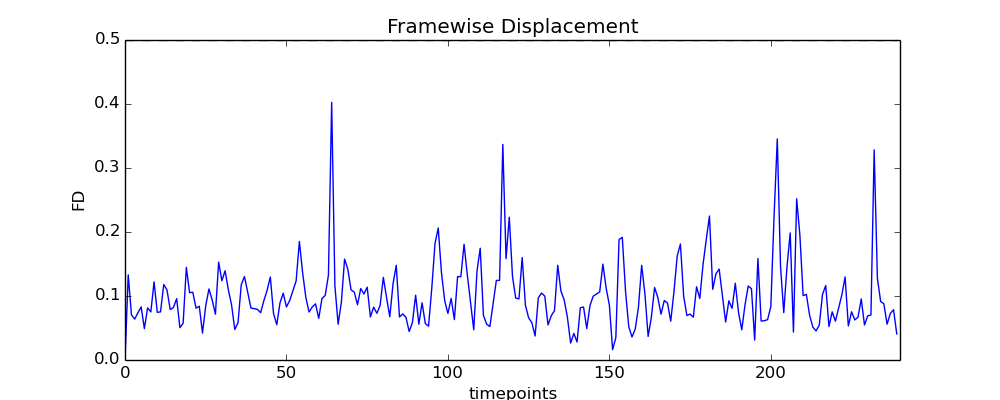
\includegraphics[scale=0.5]{figures/fd_sub2run2.png}
    \caption{Framewise Displacement for subject 2 run 2}
\end{figure}

\begin{figure}[H]
    \centering
        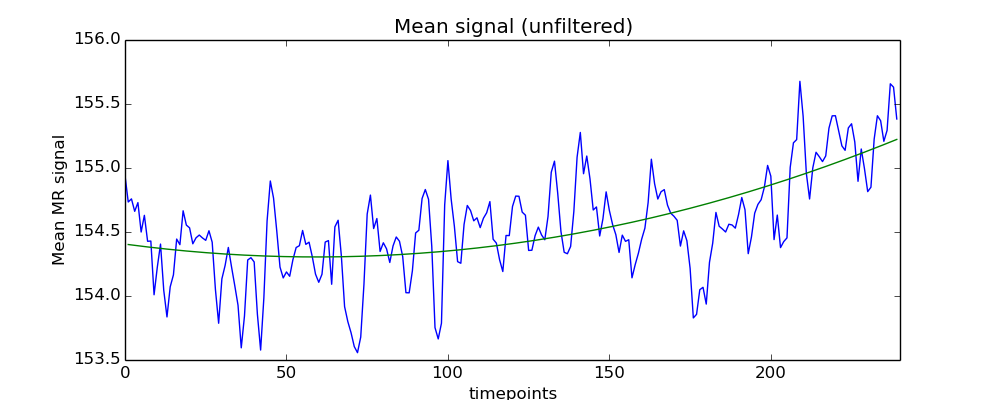
\includegraphics[scale=0.5]{figures/mean_sub2run2.png}
    \caption{Data mean for subject 2 run 2}
\end{figure}



